\documentclass[1p]{elsarticle_modified}
%\bibliographystyle{elsarticle-num}

%\usepackage[colorlinks]{hyperref}
%\usepackage{abbrmath_seonhwa} %\Abb, \Ascr, \Acal ,\Abf, \Afrak
\usepackage{amsfonts}
\usepackage{amssymb}
\usepackage{amsmath}
\usepackage{amsthm}
\usepackage{scalefnt}
\usepackage{amsbsy}
\usepackage{kotex}
\usepackage{caption}
\usepackage{subfig}
\usepackage{color}
\usepackage{graphicx}
\usepackage{xcolor} %% white, black, red, green, blue, cyan, magenta, yellow
\usepackage{float}
\usepackage{setspace}
\usepackage{hyperref}

\usepackage{tikz}
\usetikzlibrary{arrows}

\usepackage{multirow}
\usepackage{array} % fixed length table
\usepackage{hhline}

%%%%%%%%%%%%%%%%%%%%%
\makeatletter
\renewcommand*\env@matrix[1][\arraystretch]{%
	\edef\arraystretch{#1}%
	\hskip -\arraycolsep
	\let\@ifnextchar\new@ifnextchar
	\array{*\c@MaxMatrixCols c}}
\makeatother %https://tex.stackexchange.com/questions/14071/how-can-i-increase-the-line-spacing-in-a-matrix
%%%%%%%%%%%%%%%

\usepackage[normalem]{ulem}

\newcommand{\msout}[1]{\ifmmode\text{\sout{\ensuremath{#1}}}\else\sout{#1}\fi}
%SOURCE: \msout is \stkout macro in https://tex.stackexchange.com/questions/20609/strikeout-in-math-mode

\newcommand{\cancel}[1]{
	\ifmmode
	{\color{red}\msout{#1}}
	\else
	{\color{red}\sout{#1}}
	\fi
}

\newcommand{\add}[1]{
	{\color{blue}\uwave{#1}}
}

\newcommand{\replace}[2]{
	\ifmmode
	{\color{red}\msout{#1}}{\color{blue}\uwave{#2}}
	\else
	{\color{red}\sout{#1}}{\color{blue}\uwave{#2}}
	\fi
}

\newcommand{\Sol}{\mathcal{S}} %segment
\newcommand{\D}{D} %diagram
\newcommand{\A}{\mathcal{A}} %arc


%%%%%%%%%%%%%%%%%%%%%%%%%%%%%5 test

\def\sl{\operatorname{\textup{SL}}(2,\Cbb)}
\def\psl{\operatorname{\textup{PSL}}(2,\Cbb)}
\def\quan{\mkern 1mu \triangleright \mkern 1mu}

\theoremstyle{definition}
\newtheorem{thm}{Theorem}[section]
\newtheorem{prop}[thm]{Proposition}
\newtheorem{lem}[thm]{Lemma}
\newtheorem{ques}[thm]{Question}
\newtheorem{cor}[thm]{Corollary}
\newtheorem{defn}[thm]{Definition}
\newtheorem{exam}[thm]{Example}
\newtheorem{rmk}[thm]{Remark}
\newtheorem{alg}[thm]{Algorithm}

\newcommand{\I}{\sqrt{-1}}
\begin{document}

%\begin{frontmatter}
%
%\title{Boundary parabolic representations of knots up to 8 crossings}
%
%%% Group authors per affiliation:
%\author{Yunhi Cho} 
%\address{Department of Mathematics, University of Seoul, Seoul, Korea}
%\ead{yhcho@uos.ac.kr}
%
%
%\author{Seonhwa Kim} %\fnref{s_kim}}
%\address{Center for Geometry and Physics, Institute for Basic Science, Pohang, 37673, Korea}
%\ead{ryeona17@ibs.re.kr}
%
%\author{Hyuk Kim}
%\address{Department of Mathematical Sciences, Seoul National University, Seoul 08826, Korea}
%\ead{hyukkim@snu.ac.kr}
%
%\author{Seokbeom Yoon}
%\address{Department of Mathematical Sciences, Seoul National University, Seoul, 08826,  Korea}
%\ead{sbyoon15@snu.ac.kr}
%
%\begin{abstract}
%We find all boundary parabolic representation of knots up to 8 crossings.
%
%\end{abstract}
%\begin{keyword}
%    \MSC[2010] 57M25 
%\end{keyword}
%
%\end{frontmatter}

%\linenumbers
%\tableofcontents
%
\newcommand\colored[1]{\textcolor{white}{\rule[-0.35ex]{0.8em}{1.4ex}}\kern-0.8em\color{red} #1}%
%\newcommand\colored[1]{\textcolor{white}{ #1}\kern-2.17ex	\textcolor{white}{ #1}\kern-1.81ex	\textcolor{white}{ #1}\kern-2.15ex\color{red}#1	}

{\Large $\underline{12n_{0771}~(K12n_{0771})}$}

\setlength{\tabcolsep}{10pt}
\renewcommand{\arraystretch}{1.6}
\vspace{1cm}\begin{tabular}{m{100pt}>{\centering\arraybackslash}m{274pt}}
\multirow{5}{120pt}{
	\centering
	\includegraphics[width=112pt]{../../../GIT/diagram.site/Diagrams/png/2860_12n_0771.png}\\
\ \ \ A knot diagram\footnotemark}&
\allowdisplaybreaks
\textbf{Linearized knot diagam} \\
\cline{2-2}
 &
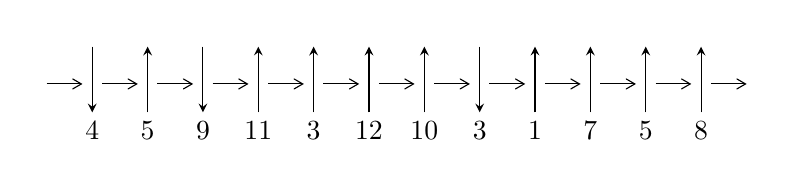
\begin{tikzpicture}[x=20pt, y=17pt]
	% nodes
	\node (C0) at (0, 0) {};
	\node (C1) at (1, 0) {};
	\node (C1U) at (1, +1) {};
	\node (C1D) at (1, -1) {4};

	\node (C2) at (2, 0) {};
	\node (C2U) at (2, +1) {};
	\node (C2D) at (2, -1) {5};

	\node (C3) at (3, 0) {};
	\node (C3U) at (3, +1) {};
	\node (C3D) at (3, -1) {9};

	\node (C4) at (4, 0) {};
	\node (C4U) at (4, +1) {};
	\node (C4D) at (4, -1) {11};

	\node (C5) at (5, 0) {};
	\node (C5U) at (5, +1) {};
	\node (C5D) at (5, -1) {3};

	\node (C6) at (6, 0) {};
	\node (C6U) at (6, +1) {};
	\node (C6D) at (6, -1) {12};

	\node (C7) at (7, 0) {};
	\node (C7U) at (7, +1) {};
	\node (C7D) at (7, -1) {10};

	\node (C8) at (8, 0) {};
	\node (C8U) at (8, +1) {};
	\node (C8D) at (8, -1) {3};

	\node (C9) at (9, 0) {};
	\node (C9U) at (9, +1) {};
	\node (C9D) at (9, -1) {1};

	\node (C10) at (10, 0) {};
	\node (C10U) at (10, +1) {};
	\node (C10D) at (10, -1) {7};

	\node (C11) at (11, 0) {};
	\node (C11U) at (11, +1) {};
	\node (C11D) at (11, -1) {5};

	\node (C12) at (12, 0) {};
	\node (C12U) at (12, +1) {};
	\node (C12D) at (12, -1) {8};
	\node (C13) at (13, 0) {};

	% arrows
	\draw[->,>={angle 60}]
	(C0) edge (C1) (C1) edge (C2) (C2) edge (C3) (C3) edge (C4) (C4) edge (C5) (C5) edge (C6) (C6) edge (C7) (C7) edge (C8) (C8) edge (C9) (C9) edge (C10) (C10) edge (C11) (C11) edge (C12) (C12) edge (C13) ;	\draw[->,>=stealth]
	(C1U) edge (C1D) (C2D) edge (C2U) (C3U) edge (C3D) (C4D) edge (C4U) (C5D) edge (C5U) (C6D) edge (C6U) (C7D) edge (C7U) (C8U) edge (C8D) (C9D) edge (C9U) (C10D) edge (C10U) (C11D) edge (C11U) (C12D) edge (C12U) ;
	\end{tikzpicture} \\
\hhline{~~} \\& 
\textbf{Solving Sequence} \\ \cline{2-2} 
 &
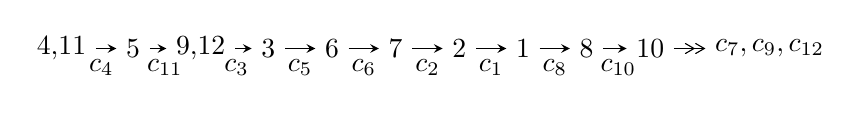
\begin{tikzpicture}[x=23pt, y=7pt]
	% node
	\node (A0) at (-1/8, 0) {4,11};
	\node (A1) at (1, 0) {5};
	\node (A2) at (33/16, 0) {9,12};
	\node (A3) at (25/8, 0) {3};
	\node (A4) at (33/8, 0) {6};
	\node (A5) at (41/8, 0) {7};
	\node (A6) at (49/8, 0) {2};
	\node (A7) at (57/8, 0) {1};
	\node (A8) at (65/8, 0) {8};
	\node (A9) at (73/8, 0) {10};
	\node (C1) at (1/2, -1) {$c_{4}$};
	\node (C2) at (3/2, -1) {$c_{11}$};
	\node (C3) at (21/8, -1) {$c_{3}$};
	\node (C4) at (29/8, -1) {$c_{5}$};
	\node (C5) at (37/8, -1) {$c_{6}$};
	\node (C6) at (45/8, -1) {$c_{2}$};
	\node (C7) at (53/8, -1) {$c_{1}$};
	\node (C8) at (61/8, -1) {$c_{8}$};
	\node (C9) at (69/8, -1) {$c_{10}$};
	\node (A10) at (11, 0) {$c_{7},c_{9},c_{12}$};

	% edge
	\draw[->,>=stealth]	
	(A0) edge (A1) (A1) edge (A2) (A2) edge (A3) (A3) edge (A4) (A4) edge (A5) (A5) edge (A6) (A6) edge (A7) (A7) edge (A8) (A8) edge (A9) ;
	\draw[->>,>={angle 60}]	
	(A9) edge (A10);
\end{tikzpicture} \\ 

\end{tabular} \\

\footnotetext{
The image of knot diagram is generated by the software ``\textbf{Draw programme}" developed by Andrew Bartholomew(\url{http://www.layer8.co.uk/maths/draw/index.htm\#Running-draw}), where we modified some parts for our purpose(\url{https://github.com/CATsTAILs/LinksPainter}).
}\phantom \\ \newline 
\centering \textbf{Ideals for irreducible components\footnotemark of $X_{\text{par}}$} 
 
\begin{align*}
I^u_{1}&=\langle 
-2.43466\times10^{230} u^{78}-1.85125\times10^{230} u^{77}+\cdots+1.68670\times10^{226} b+1.01353\times10^{231},\\
\phantom{I^u_{1}}&\phantom{= \langle  }3.16642\times10^{230} u^{78}+2.47552\times10^{230} u^{77}+\cdots+1.68670\times10^{226} a-1.45278\times10^{231},\;u^{79}+u^{78}+\cdots-23 u-1\rangle \\
I^u_{2}&=\langle 
30853 u^{27}+13876 u^{26}+\cdots+4193 b+6194,\;-17745 u^{27}-2238 u^{26}+\cdots+599 a-7171,\\
\phantom{I^u_{2}}&\phantom{= \langle  }u^{28}-9 u^{26}+\cdots- u+1\rangle \\
\\
\end{align*}
\raggedright * 2 irreducible components of $\dim_{\mathbb{C}}=0$, with total 107 representations.\\
\footnotetext{All coefficients of polynomials are rational numbers. But the coefficients are sometimes approximated in decimal forms when there is not enough margin.}
\newpage
\renewcommand{\arraystretch}{1}
\centering \section*{I. $I^u_{1}= \langle -2.43\times10^{230} u^{78}-1.85\times10^{230} u^{77}+\cdots+1.69\times10^{226} b+1.01\times10^{231},\;3.17\times10^{230} u^{78}+2.48\times10^{230} u^{77}+\cdots+1.69\times10^{226} a-1.45\times10^{231},\;u^{79}+u^{78}+\cdots-23 u-1 \rangle$}
\flushleft \textbf{(i) Arc colorings}\\
\begin{tabular}{m{7pt} m{180pt} m{7pt} m{180pt} }
\flushright $a_{4}=$&$\begin{pmatrix}1\\0\end{pmatrix}$ \\
\flushright $a_{11}=$&$\begin{pmatrix}0\\u\end{pmatrix}$ \\
\flushright $a_{5}=$&$\begin{pmatrix}1\\- u^2\end{pmatrix}$ \\
\flushright $a_{9}=$&$\begin{pmatrix}-18772.9 u^{78}-14676.7 u^{77}+\cdots+1.58492\times10^{6} u+86131.4\\14434.5 u^{78}+10975.6 u^{77}+\cdots-1.13259\times10^{6} u-60089.5\end{pmatrix}$ \\
\flushright $a_{12}=$&$\begin{pmatrix}u\\- u^3+u\end{pmatrix}$ \\
\flushright $a_{3}=$&$\begin{pmatrix}39059.0 u^{78}+30576.8 u^{77}+\cdots-3.30373\times10^{6} u-179312.\\21479.6 u^{78}+16581.0 u^{77}+\cdots-1.75206\times10^{6} u-94065.2\end{pmatrix}$ \\
\flushright $a_{6}=$&$\begin{pmatrix}-56717.2 u^{78}-43448.4 u^{77}+\cdots+4.52978\times10^{6} u+241512.\\-41302.3 u^{78}-31601.6 u^{77}+\cdots+3.29433\times10^{6} u+175706.\end{pmatrix}$ \\
\flushright $a_{7}=$&$\begin{pmatrix}-56068.0 u^{78}-42943.8 u^{77}+\cdots+4.47650\times10^{6} u+238660.\\-40684.3 u^{78}-31121.8 u^{77}+\cdots+3.24373\times10^{6} u+172999.\end{pmatrix}$ \\
\flushright $a_{2}=$&$\begin{pmatrix}15741.6 u^{78}+12555.8 u^{77}+\cdots-1.39564\times10^{6} u-76764.3\\22681.4 u^{78}+17510.4 u^{77}+\cdots-1.85056\times10^{6} u-99361.6\end{pmatrix}$ \\
\flushright $a_{1}=$&$\begin{pmatrix}38423.1 u^{78}+30066.2 u^{77}+\cdots-3.24620\times10^{6} u-176126.\\22681.4 u^{78}+17510.4 u^{77}+\cdots-1.85056\times10^{6} u-99361.6\end{pmatrix}$ \\
\flushright $a_{8}=$&$\begin{pmatrix}52534.4 u^{78}+39819.5 u^{77}+\cdots-4.08761\times10^{6} u-216260.\\28302.2 u^{78}+21431.7 u^{77}+\cdots-2.19862\times10^{6} u-116334.\end{pmatrix}$ \\
\flushright $a_{10}=$&$\begin{pmatrix}51542.3 u^{78}+39402.9 u^{77}+\cdots-4.09266\times10^{6} u-217740.\\27877.0 u^{78}+21157.7 u^{77}+\cdots-2.17777\times10^{6} u-115419.\end{pmatrix}$\\&\end{tabular}
\flushleft \textbf{(ii) Obstruction class $= -1$}\\~\\
\flushleft \textbf{(iii) Cusp Shapes $= -293314. u^{78}-224420. u^{77}+\cdots+2.33906\times10^{7} u+1.24743\times10^{6}$}\\~\\
\newpage\renewcommand{\arraystretch}{1}
\flushleft \textbf{(iv) u-Polynomials at the component}\newline \\
\begin{tabular}{m{50pt}|m{274pt}}
Crossings & \hspace{64pt}u-Polynomials at each crossing \\
\hline $$\begin{aligned}c_{1}\end{aligned}$$&$\begin{aligned}
&u^{79}-6 u^{78}+\cdots-4390196 u+145732
\end{aligned}$\\
\hline $$\begin{aligned}c_{2},c_{5}\end{aligned}$$&$\begin{aligned}
&u^{79}+6 u^{78}+\cdots-318766 u+63403
\end{aligned}$\\
\hline $$\begin{aligned}c_{3},c_{8}\end{aligned}$$&$\begin{aligned}
&u^{79}+u^{78}+\cdots-6 u-1
\end{aligned}$\\
\hline $$\begin{aligned}c_{4},c_{11}\end{aligned}$$&$\begin{aligned}
&u^{79}+u^{78}+\cdots-23 u-1
\end{aligned}$\\
\hline $$\begin{aligned}c_{6}\end{aligned}$$&$\begin{aligned}
&u^{79}- u^{78}+\cdots-3836986393 u+691687687
\end{aligned}$\\
\hline $$\begin{aligned}c_{7},c_{10}\end{aligned}$$&$\begin{aligned}
&u^{79}+3 u^{78}+\cdots+4 u+4
\end{aligned}$\\
\hline $$\begin{aligned}c_{9}\end{aligned}$$&$\begin{aligned}
&u^{79}+u^{78}+\cdots-56386 u+5447
\end{aligned}$\\
\hline $$\begin{aligned}c_{12}\end{aligned}$$&$\begin{aligned}
&u^{79}+u^{78}+\cdots-74772 u+31151
\end{aligned}$\\
\hline
\end{tabular}\\~\\
\newpage\renewcommand{\arraystretch}{1}
\flushleft \textbf{(v) Riley Polynomials at the component}\newline \\
\begin{tabular}{m{50pt}|m{274pt}}
Crossings & \hspace{64pt}Riley Polynomials at each crossing \\
\hline $$\begin{aligned}c_{1}\end{aligned}$$&$\begin{aligned}
&y^{79}-82 y^{78}+\cdots+5209547957600 y-21237815824
\end{aligned}$\\
\hline $$\begin{aligned}c_{2},c_{5}\end{aligned}$$&$\begin{aligned}
&y^{79}+82 y^{78}+\cdots+185670572514 y-4019940409
\end{aligned}$\\
\hline $$\begin{aligned}c_{3},c_{8}\end{aligned}$$&$\begin{aligned}
&y^{79}-59 y^{78}+\cdots+140 y-1
\end{aligned}$\\
\hline $$\begin{aligned}c_{4},c_{11}\end{aligned}$$&$\begin{aligned}
&y^{79}-19 y^{78}+\cdots+101 y-1
\end{aligned}$\\
\hline $$\begin{aligned}c_{6}\end{aligned}$$&$\begin{aligned}
&y^{79}+83 y^{78}+\cdots-1.11\times10^{19} y-4.78\times10^{17}
\end{aligned}$\\
\hline $$\begin{aligned}c_{7},c_{10}\end{aligned}$$&$\begin{aligned}
&y^{79}+59 y^{78}+\cdots+1152 y-16
\end{aligned}$\\
\hline $$\begin{aligned}c_{9}\end{aligned}$$&$\begin{aligned}
&y^{79}+27 y^{78}+\cdots+2658310082 y-29669809
\end{aligned}$\\
\hline $$\begin{aligned}c_{12}\end{aligned}$$&$\begin{aligned}
&y^{79}+27 y^{78}+\cdots-24342580030 y-970384801
\end{aligned}$\\
\hline
\end{tabular}\\~\\
\newpage\flushleft \textbf{(vi) Complex Volumes and Cusp Shapes}
$$\begin{array}{c|c|c}  
\text{Solutions to }I^u_{1}& \I (\text{vol} + \sqrt{-1}CS) & \text{Cusp shape}\\
 \hline 
\begin{aligned}
u &= -0.876343 + 0.418237 I \\
a &= -0.98814 + 1.09797 I \\
b &= -1.086020 - 0.390878 I\end{aligned}
 & -3.99440 - 3.41625 I & \phantom{-0.000000 } 0 \\ \hline\begin{aligned}
u &= -0.876343 - 0.418237 I \\
a &= -0.98814 - 1.09797 I \\
b &= -1.086020 + 0.390878 I\end{aligned}
 & -3.99440 + 3.41625 I & \phantom{-0.000000 } 0 \\ \hline\begin{aligned}
u &= \phantom{-}0.107309 + 1.030380 I \\
a &= \phantom{-}1.62128 - 0.02467 I \\
b &= \phantom{-}1.288120 - 0.276909 I\end{aligned}
 & -7.18782 - 0.25504 I & \phantom{-0.000000 } 0 \\ \hline\begin{aligned}
u &= \phantom{-}0.107309 - 1.030380 I \\
a &= \phantom{-}1.62128 + 0.02467 I \\
b &= \phantom{-}1.288120 + 0.276909 I\end{aligned}
 & -7.18782 + 0.25504 I & \phantom{-0.000000 } 0 \\ \hline\begin{aligned}
u &= \phantom{-}1.031440 + 0.237452 I \\
a &= \phantom{-}0.70026 - 1.45707 I \\
b &= -1.194000 + 0.073259 I\end{aligned}
 & -3.76520 - 3.47263 I & \phantom{-0.000000 } 0 \\ \hline\begin{aligned}
u &= \phantom{-}1.031440 - 0.237452 I \\
a &= \phantom{-}0.70026 + 1.45707 I \\
b &= -1.194000 - 0.073259 I\end{aligned}
 & -3.76520 + 3.47263 I & \phantom{-0.000000 } 0 \\ \hline\begin{aligned}
u &= -0.710505 + 0.791863 I \\
a &= -0.351388 + 0.386497 I \\
b &= \phantom{-}0.070718 + 0.224537 I\end{aligned}
 & -6.38277 - 1.11124 I & \phantom{-0.000000 } 0 \\ \hline\begin{aligned}
u &= -0.710505 - 0.791863 I \\
a &= -0.351388 - 0.386497 I \\
b &= \phantom{-}0.070718 - 0.224537 I\end{aligned}
 & -6.38277 + 1.11124 I & \phantom{-0.000000 } 0 \\ \hline\begin{aligned}
u &= -0.893200 + 0.104272 I \\
a &= \phantom{-}0.508013 - 0.510710 I \\
b &= \phantom{-}1.115270 + 0.582110 I\end{aligned}
 & -3.07398 - 5.47491 I & \phantom{-0.000000 } 0 \\ \hline\begin{aligned}
u &= -0.893200 - 0.104272 I \\
a &= \phantom{-}0.508013 + 0.510710 I \\
b &= \phantom{-}1.115270 - 0.582110 I\end{aligned}
 & -3.07398 + 5.47491 I & \phantom{-0.000000 } 0\\
 \hline 
 \end{array}$$\newpage$$\begin{array}{c|c|c}  
\text{Solutions to }I^u_{1}& \I (\text{vol} + \sqrt{-1}CS) & \text{Cusp shape}\\
 \hline 
\begin{aligned}
u &= \phantom{-}0.898671\phantom{ +0.000000I} \\
a &= -0.570936\phantom{ +0.000000I} \\
b &= \phantom{-}0.677206\phantom{ +0.000000I}\end{aligned}
 & \phantom{-}1.34236\phantom{ +0.000000I} & \phantom{-0.000000 } 0 \\ \hline\begin{aligned}
u &= -0.881127 + 0.684545 I \\
a &= -0.122129 - 0.303526 I \\
b &= -0.1263670 - 0.0356777 I\end{aligned}
 & -2.33613 - 2.65326 I & \phantom{-0.000000 } 0 \\ \hline\begin{aligned}
u &= -0.881127 - 0.684545 I \\
a &= -0.122129 + 0.303526 I \\
b &= -0.1263670 + 0.0356777 I\end{aligned}
 & -2.33613 + 2.65326 I & \phantom{-0.000000 } 0 \\ \hline\begin{aligned}
u &= \phantom{-}0.834574 + 0.197888 I \\
a &= \phantom{-}0.143773 + 0.431583 I \\
b &= \phantom{-}0.177668 - 0.801514 I\end{aligned}
 & -0.355058 - 0.356466 I & \phantom{-0.000000 } 0 \\ \hline\begin{aligned}
u &= \phantom{-}0.834574 - 0.197888 I \\
a &= \phantom{-}0.143773 - 0.431583 I \\
b &= \phantom{-}0.177668 + 0.801514 I\end{aligned}
 & -0.355058 + 0.356466 I & \phantom{-0.000000 } 0 \\ \hline\begin{aligned}
u &= \phantom{-}0.509087 + 0.677360 I \\
a &= \phantom{-}1.87014 + 0.09189 I \\
b &= \phantom{-}1.49340 - 0.27656 I\end{aligned}
 & -5.90433 + 7.16462 I & \phantom{-0.000000 } 0 \\ \hline\begin{aligned}
u &= \phantom{-}0.509087 - 0.677360 I \\
a &= \phantom{-}1.87014 - 0.09189 I \\
b &= \phantom{-}1.49340 + 0.27656 I\end{aligned}
 & -5.90433 - 7.16462 I & \phantom{-0.000000 } 0 \\ \hline\begin{aligned}
u &= -0.740627 + 0.409243 I \\
a &= \phantom{-}0.39635 - 1.67689 I \\
b &= \phantom{-}1.013890 + 0.493574 I\end{aligned}
 & -0.63566 - 4.72962 I & \phantom{-0.000000 } 0 \\ \hline\begin{aligned}
u &= -0.740627 - 0.409243 I \\
a &= \phantom{-}0.39635 + 1.67689 I \\
b &= \phantom{-}1.013890 - 0.493574 I\end{aligned}
 & -0.63566 + 4.72962 I & \phantom{-0.000000 } 0 \\ \hline\begin{aligned}
u &= -1.18358\phantom{ +0.000000I} \\
a &= \phantom{-}1.49313\phantom{ +0.000000I} \\
b &= \phantom{-}0.316458\phantom{ +0.000000I}\end{aligned}
 & \phantom{-}5.25090\phantom{ +0.000000I} & \phantom{-0.000000 } 0\\
 \hline 
 \end{array}$$\newpage$$\begin{array}{c|c|c}  
\text{Solutions to }I^u_{1}& \I (\text{vol} + \sqrt{-1}CS) & \text{Cusp shape}\\
 \hline 
\begin{aligned}
u &= -1.183450 + 0.177352 I \\
a &= -1.239580 - 0.395337 I \\
b &= -0.320172 + 0.018633 I\end{aligned}
 & \phantom{-}1.36097 - 5.26145 I & \phantom{-0.000000 } 0 \\ \hline\begin{aligned}
u &= -1.183450 - 0.177352 I \\
a &= -1.239580 + 0.395337 I \\
b &= -0.320172 - 0.018633 I\end{aligned}
 & \phantom{-}1.36097 + 5.26145 I & \phantom{-0.000000 } 0 \\ \hline\begin{aligned}
u &= \phantom{-}0.292091 + 0.747069 I \\
a &= -1.74758 - 0.01781 I \\
b &= -1.39008 + 0.36679 I\end{aligned}
 & -2.83896 + 3.00420 I & \phantom{-0.000000 } 0 \\ \hline\begin{aligned}
u &= \phantom{-}0.292091 - 0.747069 I \\
a &= -1.74758 + 0.01781 I \\
b &= -1.39008 - 0.36679 I\end{aligned}
 & -2.83896 - 3.00420 I & \phantom{-0.000000 } 0 \\ \hline\begin{aligned}
u &= -0.610818 + 0.485146 I \\
a &= -0.16218 + 2.43434 I \\
b &= -1.031020 - 0.463539 I\end{aligned}
 & -4.58288 - 7.29246 I & \phantom{-0.000000 } 0 \\ \hline\begin{aligned}
u &= -0.610818 - 0.485146 I \\
a &= -0.16218 - 2.43434 I \\
b &= -1.031020 + 0.463539 I\end{aligned}
 & -4.58288 + 7.29246 I & \phantom{-0.000000 } 0 \\ \hline\begin{aligned}
u &= \phantom{-}0.861534 + 0.877415 I \\
a &= -1.86321 - 0.56614 I \\
b &= -1.403680 + 0.103231 I\end{aligned}
 & -10.91540 + 5.27509 I & \phantom{-0.000000 } 0 \\ \hline\begin{aligned}
u &= \phantom{-}0.861534 - 0.877415 I \\
a &= -1.86321 + 0.56614 I \\
b &= -1.403680 - 0.103231 I\end{aligned}
 & -10.91540 - 5.27509 I & \phantom{-0.000000 } 0 \\ \hline\begin{aligned}
u &= -0.990925 + 0.780469 I \\
a &= \phantom{-}0.401539 + 0.092462 I \\
b &= \phantom{-}0.148306 - 0.099772 I\end{aligned}
 & -5.60018 - 4.78135 I & \phantom{-0.000000 } 0 \\ \hline\begin{aligned}
u &= -0.990925 - 0.780469 I \\
a &= \phantom{-}0.401539 - 0.092462 I \\
b &= \phantom{-}0.148306 + 0.099772 I\end{aligned}
 & -5.60018 + 4.78135 I & \phantom{-0.000000 } 0\\
 \hline 
 \end{array}$$\newpage$$\begin{array}{c|c|c}  
\text{Solutions to }I^u_{1}& \I (\text{vol} + \sqrt{-1}CS) & \text{Cusp shape}\\
 \hline 
\begin{aligned}
u &= \phantom{-}0.993541 + 0.817452 I \\
a &= \phantom{-}1.54937 + 1.15032 I \\
b &= \phantom{-}1.324470 - 0.054745 I\end{aligned}
 & -10.49360 + 1.06249 I & \phantom{-0.000000 } 0 \\ \hline\begin{aligned}
u &= \phantom{-}0.993541 - 0.817452 I \\
a &= \phantom{-}1.54937 - 1.15032 I \\
b &= \phantom{-}1.324470 + 0.054745 I\end{aligned}
 & -10.49360 - 1.06249 I & \phantom{-0.000000 } 0 \\ \hline\begin{aligned}
u &= \phantom{-}0.809292 + 1.039090 I \\
a &= \phantom{-}1.60729 + 0.43751 I \\
b &= \phantom{-}1.356460 - 0.150002 I\end{aligned}
 & -7.25736 + 3.90884 I & \phantom{-0.000000 } 0 \\ \hline\begin{aligned}
u &= \phantom{-}0.809292 - 1.039090 I \\
a &= \phantom{-}1.60729 - 0.43751 I \\
b &= \phantom{-}1.356460 + 0.150002 I\end{aligned}
 & -7.25736 - 3.90884 I & \phantom{-0.000000 } 0 \\ \hline\begin{aligned}
u &= \phantom{-}1.328100 + 0.137659 I \\
a &= -0.201563 + 0.611752 I \\
b &= \phantom{-}1.269440 - 0.166800 I\end{aligned}
 & \phantom{-}1.033330 + 0.782949 I & \phantom{-0.000000 } 0 \\ \hline\begin{aligned}
u &= \phantom{-}1.328100 - 0.137659 I \\
a &= -0.201563 - 0.611752 I \\
b &= \phantom{-}1.269440 + 0.166800 I\end{aligned}
 & \phantom{-}1.033330 - 0.782949 I & \phantom{-0.000000 } 0 \\ \hline\begin{aligned}
u &= -1.325470 + 0.228083 I \\
a &= \phantom{-}0.36485 - 1.74089 I \\
b &= \phantom{-}0.453543 + 1.148540 I\end{aligned}
 & \phantom{-}4.82710 - 4.04790 I & \phantom{-0.000000 } 0 \\ \hline\begin{aligned}
u &= -1.325470 - 0.228083 I \\
a &= \phantom{-}0.36485 + 1.74089 I \\
b &= \phantom{-}0.453543 - 1.148540 I\end{aligned}
 & \phantom{-}4.82710 + 4.04790 I & \phantom{-0.000000 } 0 \\ \hline\begin{aligned}
u &= \phantom{-}0.217070 + 0.610175 I \\
a &= \phantom{-}1.066590 - 0.064309 I \\
b &= -0.286678 - 0.599720 I\end{aligned}
 & -2.62047 + 3.15905 I & \phantom{-0.000000 } 0 \\ \hline\begin{aligned}
u &= \phantom{-}0.217070 - 0.610175 I \\
a &= \phantom{-}1.066590 + 0.064309 I \\
b &= -0.286678 + 0.599720 I\end{aligned}
 & -2.62047 - 3.15905 I & \phantom{-0.000000 } 0\\
 \hline 
 \end{array}$$\newpage$$\begin{array}{c|c|c}  
\text{Solutions to }I^u_{1}& \I (\text{vol} + \sqrt{-1}CS) & \text{Cusp shape}\\
 \hline 
\begin{aligned}
u &= -0.611637 + 0.124694 I \\
a &= \phantom{-}0.330543 + 0.344795 I \\
b &= -0.957604 - 0.615381 I\end{aligned}
 & -0.97782 - 3.18704 I & \phantom{-0.000000 } 0 \\ \hline\begin{aligned}
u &= -0.611637 - 0.124694 I \\
a &= \phantom{-}0.330543 - 0.344795 I \\
b &= -0.957604 + 0.615381 I\end{aligned}
 & -0.97782 + 3.18704 I & \phantom{-0.000000 } 0 \\ \hline\begin{aligned}
u &= \phantom{-}0.983833 + 0.979662 I \\
a &= \phantom{-}0.537912 + 0.047191 I \\
b &= \phantom{-}0.017508 - 1.337210 I\end{aligned}
 & -8.04470 + 9.99314 I & \phantom{-0.000000 } 0 \\ \hline\begin{aligned}
u &= \phantom{-}0.983833 - 0.979662 I \\
a &= \phantom{-}0.537912 - 0.047191 I \\
b &= \phantom{-}0.017508 + 1.337210 I\end{aligned}
 & -8.04470 - 9.99314 I & \phantom{-0.000000 } 0 \\ \hline\begin{aligned}
u &= -0.784345 + 1.145680 I \\
a &= \phantom{-}1.002190 - 0.273503 I \\
b &= \phantom{-}1.60552 - 0.59569 I\end{aligned}
 & -13.07230 - 2.79558 I & \phantom{-0.000000 } 0 \\ \hline\begin{aligned}
u &= -0.784345 - 1.145680 I \\
a &= \phantom{-}1.002190 + 0.273503 I \\
b &= \phantom{-}1.60552 + 0.59569 I\end{aligned}
 & -13.07230 + 2.79558 I & \phantom{-0.000000 } 0 \\ \hline\begin{aligned}
u &= \phantom{-}0.361058 + 0.488552 I \\
a &= -0.921454 - 0.696855 I \\
b &= -0.669008 + 0.782264 I\end{aligned}
 & \phantom{-}0.17362 + 2.13315 I & \phantom{-0.000000 } 0 \\ \hline\begin{aligned}
u &= \phantom{-}0.361058 - 0.488552 I \\
a &= -0.921454 + 0.696855 I \\
b &= -0.669008 - 0.782264 I\end{aligned}
 & \phantom{-}0.17362 - 2.13315 I & \phantom{-0.000000 } 0 \\ \hline\begin{aligned}
u &= \phantom{-}1.008820 + 0.976571 I \\
a &= \phantom{-}0.568830 + 0.028624 I \\
b &= -0.277407 - 1.304630 I\end{aligned}
 & -7.98302 - 2.79382 I & \phantom{-0.000000 } 0 \\ \hline\begin{aligned}
u &= \phantom{-}1.008820 - 0.976571 I \\
a &= \phantom{-}0.568830 - 0.028624 I \\
b &= -0.277407 + 1.304630 I\end{aligned}
 & -7.98302 + 2.79382 I & \phantom{-0.000000 } 0\\
 \hline 
 \end{array}$$\newpage$$\begin{array}{c|c|c}  
\text{Solutions to }I^u_{1}& \I (\text{vol} + \sqrt{-1}CS) & \text{Cusp shape}\\
 \hline 
\begin{aligned}
u &= \phantom{-}0.531319 + 0.254208 I \\
a &= -0.764712 - 0.499735 I \\
b &= \phantom{-}0.413560 + 0.543062 I\end{aligned}
 & \phantom{-}1.055930 + 0.468133 I & \phantom{-0.000000 } 0 \\ \hline\begin{aligned}
u &= \phantom{-}0.531319 - 0.254208 I \\
a &= -0.764712 + 0.499735 I \\
b &= \phantom{-}0.413560 - 0.543062 I\end{aligned}
 & \phantom{-}1.055930 - 0.468133 I & \phantom{-0.000000 } 0 \\ \hline\begin{aligned}
u &= \phantom{-}0.99618 + 1.02534 I \\
a &= -0.559912 - 0.038895 I \\
b &= \phantom{-}0.10002 + 1.47274 I\end{aligned}
 & -3.23697 + 3.73023 I & \phantom{-0.000000 } 0 \\ \hline\begin{aligned}
u &= \phantom{-}0.99618 - 1.02534 I \\
a &= -0.559912 + 0.038895 I \\
b &= \phantom{-}0.10002 - 1.47274 I\end{aligned}
 & -3.23697 - 3.73023 I & \phantom{-0.000000 } 0 \\ \hline\begin{aligned}
u &= -0.81627 + 1.20218 I \\
a &= -1.047240 + 0.299529 I \\
b &= -1.60684 + 0.48551 I\end{aligned}
 & -9.14876 + 3.35329 I & \phantom{-0.000000 } 0 \\ \hline\begin{aligned}
u &= -0.81627 - 1.20218 I \\
a &= -1.047240 - 0.299529 I \\
b &= -1.60684 - 0.48551 I\end{aligned}
 & -9.14876 - 3.35329 I & \phantom{-0.000000 } 0 \\ \hline\begin{aligned}
u &= \phantom{-}1.13111 + 0.92779 I \\
a &= -1.25926 - 0.81035 I \\
b &= -1.306360 + 0.089703 I\end{aligned}
 & -6.27013 + 3.29120 I & \phantom{-0.000000 } 0 \\ \hline\begin{aligned}
u &= \phantom{-}1.13111 - 0.92779 I \\
a &= -1.25926 + 0.81035 I \\
b &= -1.306360 - 0.089703 I\end{aligned}
 & -6.27013 - 3.29120 I & \phantom{-0.000000 } 0 \\ \hline\begin{aligned}
u &= -0.85049 + 1.21862 I \\
a &= \phantom{-}1.080010 - 0.274442 I \\
b &= \phantom{-}1.53645 - 0.46171 I\end{aligned}
 & -13.8996 + 8.9563 I & \phantom{-0.000000 } 0 \\ \hline\begin{aligned}
u &= -0.85049 - 1.21862 I \\
a &= \phantom{-}1.080010 + 0.274442 I \\
b &= \phantom{-}1.53645 + 0.46171 I\end{aligned}
 & -13.8996 - 8.9563 I & \phantom{-0.000000 } 0\\
 \hline 
 \end{array}$$\newpage$$\begin{array}{c|c|c}  
\text{Solutions to }I^u_{1}& \I (\text{vol} + \sqrt{-1}CS) & \text{Cusp shape}\\
 \hline 
\begin{aligned}
u &= -0.439096 + 0.241787 I \\
a &= -2.48467 - 0.16848 I \\
b &= \phantom{-}0.817333 + 0.425600 I\end{aligned}
 & -6.30949 - 1.87842 I & \phantom{-0.000000 -}0. + 3.28089 I \\ \hline\begin{aligned}
u &= -0.439096 - 0.241787 I \\
a &= -2.48467 + 0.16848 I \\
b &= \phantom{-}0.817333 - 0.425600 I\end{aligned}
 & -6.30949 + 1.87842 I & \phantom{-0.000000 } 0. - 3.28089 I \\ \hline\begin{aligned}
u &= -1.20607 + 0.92056 I \\
a &= -1.08447 + 1.12933 I \\
b &= -1.48840 - 0.74155 I\end{aligned}
 & -11.71210 - 4.71803 I & \phantom{-0.000000 } 0 \\ \hline\begin{aligned}
u &= -1.20607 - 0.92056 I \\
a &= -1.08447 - 1.12933 I \\
b &= -1.48840 + 0.74155 I\end{aligned}
 & -11.71210 + 4.71803 I & \phantom{-0.000000 } 0 \\ \hline\begin{aligned}
u &= -1.17728 + 0.96277 I \\
a &= -1.24134 + 1.03090 I \\
b &= -1.46917 - 0.60570 I\end{aligned}
 & -12.7672 - 16.7760 I & \phantom{-0.000000 } 0 \\ \hline\begin{aligned}
u &= -1.17728 - 0.96277 I \\
a &= -1.24134 - 1.03090 I \\
b &= -1.46917 + 0.60570 I\end{aligned}
 & -12.7672 + 16.7760 I & \phantom{-0.000000 } 0 \\ \hline\begin{aligned}
u &= -1.18703 + 0.95708 I \\
a &= \phantom{-}1.16866 - 1.03328 I \\
b &= \phantom{-}1.50856 + 0.63733 I\end{aligned}
 & -7.92089 - 11.10750 I & \phantom{-0.000000 } 0 \\ \hline\begin{aligned}
u &= -1.18703 - 0.95708 I \\
a &= \phantom{-}1.16866 + 1.03328 I \\
b &= \phantom{-}1.50856 - 0.63733 I\end{aligned}
 & -7.92089 + 11.10750 I & \phantom{-0.000000 } 0 \\ \hline\begin{aligned}
u &= \phantom{-}1.51003 + 0.36636 I \\
a &= -0.299045 - 0.591632 I \\
b &= -1.293010 + 0.090598 I\end{aligned}
 & -2.23461 + 5.90245 I & \phantom{-0.000000 } 0 \\ \hline\begin{aligned}
u &= \phantom{-}1.51003 - 0.36636 I \\
a &= -0.299045 + 0.591632 I \\
b &= -1.293010 - 0.090598 I\end{aligned}
 & -2.23461 - 5.90245 I & \phantom{-0.000000 } 0\\
 \hline 
 \end{array}$$\newpage$$\begin{array}{c|c|c}  
\text{Solutions to }I^u_{1}& \I (\text{vol} + \sqrt{-1}CS) & \text{Cusp shape}\\
 \hline 
\begin{aligned}
u &= \phantom{-}0.79204 + 1.35981 I \\
a &= -1.40007 - 0.29591 I \\
b &= -1.301060 + 0.173804 I\end{aligned}
 & -10.67170 + 2.96611 I & \phantom{-0.000000 } 0 \\ \hline\begin{aligned}
u &= \phantom{-}0.79204 - 1.35981 I \\
a &= -1.40007 + 0.29591 I \\
b &= -1.301060 - 0.173804 I\end{aligned}
 & -10.67170 - 2.96611 I & \phantom{-0.000000 } 0 \\ \hline\begin{aligned}
u &= \phantom{-}1.24583 + 1.16094 I \\
a &= \phantom{-}1.176150 + 0.530089 I \\
b &= \phantom{-}1.286220 - 0.113435 I\end{aligned}
 & -9.34277 + 5.87011 I & \phantom{-0.000000 } 0 \\ \hline\begin{aligned}
u &= \phantom{-}1.24583 - 1.16094 I \\
a &= \phantom{-}1.176150 - 0.530089 I \\
b &= \phantom{-}1.286220 + 0.113435 I\end{aligned}
 & -9.34277 - 5.87011 I & \phantom{-0.000000 } 0 \\ \hline\begin{aligned}
u &= -0.271329 + 0.031654 I \\
a &= -8.02705 + 3.97881 I \\
b &= -0.749966 + 0.052776 I\end{aligned}
 & -2.06804 - 3.78913 I & -2.03961 + 6.55169 I \\ \hline\begin{aligned}
u &= -0.271329 - 0.031654 I \\
a &= -8.02705 - 3.97881 I \\
b &= -0.749966 - 0.052776 I\end{aligned}
 & -2.06804 + 3.78913 I & -2.03961 - 6.55169 I \\ \hline\begin{aligned}
u &= -0.234685 + 0.005537 I \\
a &= \phantom{-}0.13366 + 1.71141 I \\
b &= -0.396879 + 1.158900 I\end{aligned}
 & \phantom{-}0.89026 + 2.40339 I & -0.5139 - 16.4120 I \\ \hline\begin{aligned}
u &= -0.234685 - 0.005537 I \\
a &= \phantom{-}0.13366 - 1.71141 I \\
b &= -0.396879 - 1.158900 I\end{aligned}
 & \phantom{-}0.89026 - 2.40339 I & -0.5139 + 16.4120 I \\ \hline\begin{aligned}
u &= -0.222199\phantom{ +0.000000I} \\
a &= \phantom{-}9.15297\phantom{ +0.000000I} \\
b &= \phantom{-}0.720846\phantom{ +0.000000I}\end{aligned}
 & \phantom{-}1.95313\phantom{ +0.000000I} & \phantom{-}2.25730\phantom{ +0.000000I}\\
 \hline 
 \end{array}$$\newpage\newpage\renewcommand{\arraystretch}{1}
\centering \section*{II. $I^u_{2}= \langle 30853 u^{27}+13876 u^{26}+\cdots+4193 b+6194,\;-17745 u^{27}-2238 u^{26}+\cdots+599 a-7171,\;u^{28}-9 u^{26}+\cdots- u+1 \rangle$}
\flushleft \textbf{(i) Arc colorings}\\
\begin{tabular}{m{7pt} m{180pt} m{7pt} m{180pt} }
\flushright $a_{4}=$&$\begin{pmatrix}1\\0\end{pmatrix}$ \\
\flushright $a_{11}=$&$\begin{pmatrix}0\\u\end{pmatrix}$ \\
\flushright $a_{5}=$&$\begin{pmatrix}1\\- u^2\end{pmatrix}$ \\
\flushright $a_{9}=$&$\begin{pmatrix}29.6244 u^{27}+3.73623 u^{26}+\cdots-69.0184 u+11.9716\\-7.35822 u^{27}-3.30933 u^{26}+\cdots+12.9685 u-1.47722\end{pmatrix}$ \\
\flushright $a_{12}=$&$\begin{pmatrix}u\\- u^3+u\end{pmatrix}$ \\
\flushright $a_{3}=$&$\begin{pmatrix}-1.13809 u^{27}-18.3236 u^{26}+\cdots-50.6220 u+61.0258\\-1.73718 u^{27}+5.35345 u^{26}+\cdots+29.1855 u-17.3236\end{pmatrix}$ \\
\flushright $a_{6}=$&$\begin{pmatrix}42.7021 u^{27}+1.87527 u^{26}+\cdots-129.214 u-8.26568\\-11.9702 u^{27}+0.798712 u^{26}+\cdots+38.8269 u-10.1247\end{pmatrix}$ \\
\flushright $a_{7}=$&$\begin{pmatrix}29.7319 u^{27}+1.67398 u^{26}+\cdots-88.3871 u-7.39041\\-21.0835 u^{27}+0.163606 u^{26}+\cdots+66.8848 u-9.45075\end{pmatrix}$ \\
\flushright $a_{2}=$&$\begin{pmatrix}-0.138087 u^{27}-18.3236 u^{26}+\cdots-62.6220 u+60.0258\\-1.73718 u^{27}+5.35345 u^{26}+\cdots+30.1855 u-17.3236\end{pmatrix}$ \\
\flushright $a_{1}=$&$\begin{pmatrix}-1.87527 u^{27}-12.9702 u^{26}+\cdots-32.4364 u+42.7021\\-1.73718 u^{27}+5.35345 u^{26}+\cdots+30.1855 u-17.3236\end{pmatrix}$ \\
\flushright $a_{8}=$&$\begin{pmatrix}8.52278 u^{27}+11.3582 u^{26}+\cdots+4.71572 u-25.4913\\8.31600 u^{27}-7.33365 u^{26}+\cdots-52.6353 u+10.2778\end{pmatrix}$ \\
\flushright $a_{10}=$&$\begin{pmatrix}16.5900 u^{27}+17.5521 u^{26}+\cdots+20.1171 u-48.1567\\-17.1283 u^{27}+3.03434 u^{26}+\cdots+38.6172 u-20.0072\end{pmatrix}$\\&\end{tabular}
\flushleft \textbf{(ii) Obstruction class $= 1$}\\~\\
\flushleft \textbf{(iii) Cusp Shapes $= -\frac{14948}{4193} u^{27}-\frac{188690}{4193} u^{26}+\cdots-\frac{332851}{4193} u+\frac{609209}{4193}$}\\~\\
\newpage\renewcommand{\arraystretch}{1}
\flushleft \textbf{(iv) u-Polynomials at the component}\newline \\
\begin{tabular}{m{50pt}|m{274pt}}
Crossings & \hspace{64pt}u-Polynomials at each crossing \\
\hline $$\begin{aligned}c_{1}\end{aligned}$$&$\begin{aligned}
&u^{28}-11 u^{27}+\cdots-72 u-4
\end{aligned}$\\
\hline $$\begin{aligned}c_{2}\end{aligned}$$&$\begin{aligned}
&u^{28}+u^{27}+\cdots+8 u^2-1
\end{aligned}$\\
\hline $$\begin{aligned}c_{3}\end{aligned}$$&$\begin{aligned}
&u^{28}-7 u^{26}+\cdots+9 u^2-1
\end{aligned}$\\
\hline $$\begin{aligned}c_{4}\end{aligned}$$&$\begin{aligned}
&u^{28}-9 u^{26}+\cdots- u+1
\end{aligned}$\\
\hline $$\begin{aligned}c_{5}\end{aligned}$$&$\begin{aligned}
&u^{28}- u^{27}+\cdots+8 u^2-1
\end{aligned}$\\
\hline $$\begin{aligned}c_{6}\end{aligned}$$&$\begin{aligned}
&u^{28}+8 u^{26}+\cdots+57 u-107
\end{aligned}$\\
\hline $$\begin{aligned}c_{7}\end{aligned}$$&$\begin{aligned}
&u^{28}+4 u^{27}+\cdots+8 u+4
\end{aligned}$\\
\hline $$\begin{aligned}c_{8}\end{aligned}$$&$\begin{aligned}
&u^{28}-7 u^{26}+\cdots+9 u^2-1
\end{aligned}$\\
\hline $$\begin{aligned}c_{9}\end{aligned}$$&$\begin{aligned}
&u^{28}+4 u^{25}+\cdots-4 u-1
\end{aligned}$\\
\hline $$\begin{aligned}c_{10}\end{aligned}$$&$\begin{aligned}
&u^{28}-4 u^{27}+\cdots-8 u+4
\end{aligned}$\\
\hline $$\begin{aligned}c_{11}\end{aligned}$$&$\begin{aligned}
&u^{28}-9 u^{26}+\cdots+u+1
\end{aligned}$\\
\hline $$\begin{aligned}c_{12}\end{aligned}$$&$\begin{aligned}
&u^{28}-2 u^{26}+\cdots-12 u^2-1
\end{aligned}$\\
\hline
\end{tabular}\\~\\
\newpage\renewcommand{\arraystretch}{1}
\flushleft \textbf{(v) Riley Polynomials at the component}\newline \\
\begin{tabular}{m{50pt}|m{274pt}}
Crossings & \hspace{64pt}Riley Polynomials at each crossing \\
\hline $$\begin{aligned}c_{1}\end{aligned}$$&$\begin{aligned}
&y^{28}-25 y^{27}+\cdots-3120 y+16
\end{aligned}$\\
\hline $$\begin{aligned}c_{2},c_{5}\end{aligned}$$&$\begin{aligned}
&y^{28}+11 y^{27}+\cdots-16 y+1
\end{aligned}$\\
\hline $$\begin{aligned}c_{3},c_{8}\end{aligned}$$&$\begin{aligned}
&y^{28}-14 y^{27}+\cdots-18 y+1
\end{aligned}$\\
\hline $$\begin{aligned}c_{4},c_{11}\end{aligned}$$&$\begin{aligned}
&y^{28}-18 y^{27}+\cdots-27 y+1
\end{aligned}$\\
\hline $$\begin{aligned}c_{6}\end{aligned}$$&$\begin{aligned}
&y^{28}+16 y^{27}+\cdots-141921 y+11449
\end{aligned}$\\
\hline $$\begin{aligned}c_{7},c_{10}\end{aligned}$$&$\begin{aligned}
&y^{28}+20 y^{27}+\cdots+80 y+16
\end{aligned}$\\
\hline $$\begin{aligned}c_{9}\end{aligned}$$&$\begin{aligned}
&y^{28}+24 y^{26}+\cdots+16 y+1
\end{aligned}$\\
\hline $$\begin{aligned}c_{12}\end{aligned}$$&$\begin{aligned}
&y^{28}-4 y^{27}+\cdots+24 y+1
\end{aligned}$\\
\hline
\end{tabular}\\~\\
\newpage\flushleft \textbf{(vi) Complex Volumes and Cusp Shapes}
$$\begin{array}{c|c|c}  
\text{Solutions to }I^u_{2}& \I (\text{vol} + \sqrt{-1}CS) & \text{Cusp shape}\\
 \hline 
\begin{aligned}
u &= -0.852125 + 0.601245 I \\
a &= -0.832108 - 0.231328 I \\
b &= \phantom{-}0.747853 - 0.466030 I\end{aligned}
 & -6.71180 + 0.04614 I & -0.064629 - 0.987396 I \\ \hline\begin{aligned}
u &= -0.852125 - 0.601245 I \\
a &= -0.832108 + 0.231328 I \\
b &= \phantom{-}0.747853 + 0.466030 I\end{aligned}
 & -6.71180 - 0.04614 I & -0.064629 + 0.987396 I \\ \hline\begin{aligned}
u &= -0.854084 + 0.782815 I \\
a &= \phantom{-}0.436404 - 0.146646 I \\
b &= \phantom{-}0.155074 + 0.739479 I\end{aligned}
 & -1.77839 - 2.94686 I & \phantom{-}9.10140 + 4.88751 I \\ \hline\begin{aligned}
u &= -0.854084 - 0.782815 I \\
a &= \phantom{-}0.436404 + 0.146646 I \\
b &= \phantom{-}0.155074 - 0.739479 I\end{aligned}
 & -1.77839 + 2.94686 I & \phantom{-}9.10140 - 4.88751 I \\ \hline\begin{aligned}
u &= -0.971333 + 0.742339 I \\
a &= -0.197178 + 0.525278 I \\
b &= -0.699311 - 0.194741 I\end{aligned}
 & -6.17700 - 5.22730 I & -3.13585 + 7.30911 I \\ \hline\begin{aligned}
u &= -0.971333 - 0.742339 I \\
a &= -0.197178 - 0.525278 I \\
b &= -0.699311 + 0.194741 I\end{aligned}
 & -6.17700 + 5.22730 I & -3.13585 - 7.30911 I \\ \hline\begin{aligned}
u &= \phantom{-}1.22488\phantom{ +0.000000I} \\
a &= -1.38709\phantom{ +0.000000I} \\
b &= -0.689063\phantom{ +0.000000I}\end{aligned}
 & \phantom{-}4.80480\phantom{ +0.000000I} & \phantom{-}3.24890\phantom{ +0.000000I} \\ \hline\begin{aligned}
u &= \phantom{-}1.232920 + 0.196608 I \\
a &= \phantom{-}1.290190 - 0.099792 I \\
b &= \phantom{-}0.741690 + 0.131648 I\end{aligned}
 & \phantom{-}0.83876 + 4.91408 I & \phantom{-}1.44350 - 1.61325 I \\ \hline\begin{aligned}
u &= \phantom{-}1.232920 - 0.196608 I \\
a &= \phantom{-}1.290190 + 0.099792 I \\
b &= \phantom{-}0.741690 - 0.131648 I\end{aligned}
 & \phantom{-}0.83876 - 4.91408 I & \phantom{-}1.44350 + 1.61325 I \\ \hline\begin{aligned}
u &= -0.655111 + 0.359817 I \\
a &= \phantom{-}0.659090 - 0.948985 I \\
b &= \phantom{-}1.048160 + 0.626210 I\end{aligned}
 & -1.19938 - 3.96368 I & \phantom{-}5.40589 + 6.56623 I\\
 \hline 
 \end{array}$$\newpage$$\begin{array}{c|c|c}  
\text{Solutions to }I^u_{2}& \I (\text{vol} + \sqrt{-1}CS) & \text{Cusp shape}\\
 \hline 
\begin{aligned}
u &= -0.655111 - 0.359817 I \\
a &= \phantom{-}0.659090 + 0.948985 I \\
b &= \phantom{-}1.048160 - 0.626210 I\end{aligned}
 & -1.19938 + 3.96368 I & \phantom{-}5.40589 - 6.56623 I \\ \hline\begin{aligned}
u &= -1.263940 + 0.151253 I \\
a &= \phantom{-}0.368613 - 0.364180 I \\
b &= -1.236920 + 0.502499 I\end{aligned}
 & \phantom{-}1.20025 + 1.95116 I & \phantom{-}6.65433 - 3.75191 I \\ \hline\begin{aligned}
u &= -1.263940 - 0.151253 I \\
a &= \phantom{-}0.368613 + 0.364180 I \\
b &= -1.236920 - 0.502499 I\end{aligned}
 & \phantom{-}1.20025 - 1.95116 I & \phantom{-}6.65433 + 3.75191 I \\ \hline\begin{aligned}
u &= -1.301720 + 0.177857 I \\
a &= -0.033564 - 0.438214 I \\
b &= \phantom{-}1.132780 + 0.311775 I\end{aligned}
 & -0.95254 - 6.85547 I & \phantom{-}6.26006 + 7.50495 I \\ \hline\begin{aligned}
u &= -1.301720 - 0.177857 I \\
a &= -0.033564 + 0.438214 I \\
b &= \phantom{-}1.132780 - 0.311775 I\end{aligned}
 & -0.95254 + 6.85547 I & \phantom{-}6.26006 - 7.50495 I \\ \hline\begin{aligned}
u &= \phantom{-}0.661543\phantom{ +0.000000I} \\
a &= -2.96465\phantom{ +0.000000I} \\
b &= \phantom{-}0.557034\phantom{ +0.000000I}\end{aligned}
 & \phantom{-}2.52967\phantom{ +0.000000I} & \phantom{-}18.0280\phantom{ +0.000000I} \\ \hline\begin{aligned}
u &= \phantom{-}0.632952 + 0.113297 I \\
a &= \phantom{-}2.91957 - 3.06599 I \\
b &= -0.637106 + 0.134427 I\end{aligned}
 & -1.64115 - 3.51490 I & \phantom{-}12.07415 - 1.40885 I \\ \hline\begin{aligned}
u &= \phantom{-}0.632952 - 0.113297 I \\
a &= \phantom{-}2.91957 + 3.06599 I \\
b &= -0.637106 - 0.134427 I\end{aligned}
 & -1.64115 + 3.51490 I & \phantom{-}12.07415 + 1.40885 I \\ \hline\begin{aligned}
u &= \phantom{-}0.905198 + 1.014880 I \\
a &= \phantom{-}1.58689 + 0.69818 I \\
b &= \phantom{-}1.315490 - 0.237768 I\end{aligned}
 & -9.20708 + 3.02208 I & \phantom{-}0.86618 - 2.28131 I \\ \hline\begin{aligned}
u &= \phantom{-}0.905198 - 1.014880 I \\
a &= \phantom{-}1.58689 - 0.69818 I \\
b &= \phantom{-}1.315490 + 0.237768 I\end{aligned}
 & -9.20708 - 3.02208 I & \phantom{-}0.86618 + 2.28131 I\\
 \hline 
 \end{array}$$\newpage$$\begin{array}{c|c|c}  
\text{Solutions to }I^u_{2}& \I (\text{vol} + \sqrt{-1}CS) & \text{Cusp shape}\\
 \hline 
\begin{aligned}
u &= \phantom{-}1.358480 + 0.221950 I \\
a &= -0.29847 - 1.70421 I \\
b &= -0.427126 + 1.219380 I\end{aligned}
 & \phantom{-}4.68108 + 4.11341 I & -14.1729 - 14.5736 I \\ \hline\begin{aligned}
u &= \phantom{-}1.358480 - 0.221950 I \\
a &= -0.29847 + 1.70421 I \\
b &= -0.427126 - 1.219380 I\end{aligned}
 & \phantom{-}4.68108 - 4.11341 I & -14.1729 + 14.5736 I \\ \hline\begin{aligned}
u &= -0.565004 + 0.040165 I \\
a &= -0.26511 + 2.40588 I \\
b &= -1.181360 - 0.443555 I\end{aligned}
 & -4.21817 - 6.13927 I & \phantom{-}2.12135 + 6.27361 I \\ \hline\begin{aligned}
u &= -0.565004 - 0.040165 I \\
a &= -0.26511 - 2.40588 I \\
b &= -1.181360 + 0.443555 I\end{aligned}
 & -4.21817 + 6.13927 I & \phantom{-}2.12135 - 6.27361 I \\ \hline\begin{aligned}
u &= \phantom{-}0.93379 + 1.09566 I \\
a &= -1.43251 - 0.41148 I \\
b &= -1.334820 + 0.045448 I\end{aligned}
 & -9.12029 + 4.54261 I & \phantom{-0.000000 } 0. - 2.64613 I \\ \hline\begin{aligned}
u &= \phantom{-}0.93379 - 1.09566 I \\
a &= -1.43251 + 0.41148 I \\
b &= -1.334820 - 0.045448 I\end{aligned}
 & -9.12029 - 4.54261 I & \phantom{-0.000000 -}0. + 2.64613 I \\ \hline\begin{aligned}
u &= \phantom{-}0.456757 + 0.180125 I \\
a &= \phantom{-}0.474060 + 0.395975 I \\
b &= \phantom{-}0.441601 + 1.138690 I\end{aligned}
 & \phantom{-}1.00966 - 2.17421 I & \phantom{-}13.7438 - 10.2319 I \\ \hline\begin{aligned}
u &= \phantom{-}0.456757 - 0.180125 I \\
a &= \phantom{-}0.474060 - 0.395975 I \\
b &= \phantom{-}0.441601 - 1.138690 I\end{aligned}
 & \phantom{-}1.00966 + 2.17421 I & \phantom{-}13.7438 + 10.2319 I\\
 \hline 
 \end{array}$$\newpage
\newpage\renewcommand{\arraystretch}{1}
\centering \section*{ III. u-Polynomials}
\begin{tabular}{m{50pt}|m{274pt}}
Crossings & \hspace{64pt}u-Polynomials at each crossing \\
\hline $$\begin{aligned}c_{1}\end{aligned}$$&$\begin{aligned}
&(u^{28}-11 u^{27}+\cdots-72 u-4)(u^{79}-6 u^{78}+\cdots-4390196 u+145732)
\end{aligned}$\\
\hline $$\begin{aligned}c_{2}\end{aligned}$$&$\begin{aligned}
&(u^{28}+u^{27}+\cdots+8 u^2-1)(u^{79}+6 u^{78}+\cdots-318766 u+63403)
\end{aligned}$\\
\hline $$\begin{aligned}c_{3}\end{aligned}$$&$\begin{aligned}
&(u^{28}-7 u^{26}+\cdots+9 u^2-1)(u^{79}+u^{78}+\cdots-6 u-1)
\end{aligned}$\\
\hline $$\begin{aligned}c_{4}\end{aligned}$$&$\begin{aligned}
&(u^{28}-9 u^{26}+\cdots- u+1)(u^{79}+u^{78}+\cdots-23 u-1)
\end{aligned}$\\
\hline $$\begin{aligned}c_{5}\end{aligned}$$&$\begin{aligned}
&(u^{28}- u^{27}+\cdots+8 u^2-1)(u^{79}+6 u^{78}+\cdots-318766 u+63403)
\end{aligned}$\\
\hline $$\begin{aligned}c_{6}\end{aligned}$$&$\begin{aligned}
&(u^{28}+8 u^{26}+\cdots+57 u-107)\\
&\cdot(u^{79}- u^{78}+\cdots-3836986393 u+691687687)
\end{aligned}$\\
\hline $$\begin{aligned}c_{7}\end{aligned}$$&$\begin{aligned}
&(u^{28}+4 u^{27}+\cdots+8 u+4)(u^{79}+3 u^{78}+\cdots+4 u+4)
\end{aligned}$\\
\hline $$\begin{aligned}c_{8}\end{aligned}$$&$\begin{aligned}
&(u^{28}-7 u^{26}+\cdots+9 u^2-1)(u^{79}+u^{78}+\cdots-6 u-1)
\end{aligned}$\\
\hline $$\begin{aligned}c_{9}\end{aligned}$$&$\begin{aligned}
&(u^{28}+4 u^{25}+\cdots-4 u-1)(u^{79}+u^{78}+\cdots-56386 u+5447)
\end{aligned}$\\
\hline $$\begin{aligned}c_{10}\end{aligned}$$&$\begin{aligned}
&(u^{28}-4 u^{27}+\cdots-8 u+4)(u^{79}+3 u^{78}+\cdots+4 u+4)
\end{aligned}$\\
\hline $$\begin{aligned}c_{11}\end{aligned}$$&$\begin{aligned}
&(u^{28}-9 u^{26}+\cdots+u+1)(u^{79}+u^{78}+\cdots-23 u-1)
\end{aligned}$\\
\hline $$\begin{aligned}c_{12}\end{aligned}$$&$\begin{aligned}
&(u^{28}-2 u^{26}+\cdots-12 u^2-1)(u^{79}+u^{78}+\cdots-74772 u+31151)
\end{aligned}$\\
\hline
\end{tabular}\newpage\renewcommand{\arraystretch}{1}
\centering \section*{ IV. Riley Polynomials}
\begin{tabular}{m{50pt}|m{274pt}}
Crossings & \hspace{64pt}Riley Polynomials at each crossing \\
\hline $$\begin{aligned}c_{1}\end{aligned}$$&$\begin{aligned}
&(y^{28}-25 y^{27}+\cdots-3120 y+16)\\
&\cdot(y^{79}-82 y^{78}+\cdots+5209547957600 y-21237815824)
\end{aligned}$\\
\hline $$\begin{aligned}c_{2},c_{5}\end{aligned}$$&$\begin{aligned}
&(y^{28}+11 y^{27}+\cdots-16 y+1)\\
&\cdot(y^{79}+82 y^{78}+\cdots+185670572514 y-4019940409)
\end{aligned}$\\
\hline $$\begin{aligned}c_{3},c_{8}\end{aligned}$$&$\begin{aligned}
&(y^{28}-14 y^{27}+\cdots-18 y+1)(y^{79}-59 y^{78}+\cdots+140 y-1)
\end{aligned}$\\
\hline $$\begin{aligned}c_{4},c_{11}\end{aligned}$$&$\begin{aligned}
&(y^{28}-18 y^{27}+\cdots-27 y+1)(y^{79}-19 y^{78}+\cdots+101 y-1)
\end{aligned}$\\
\hline $$\begin{aligned}c_{6}\end{aligned}$$&$\begin{aligned}
&(y^{28}+16 y^{27}+\cdots-141921 y+11449)\\
&\cdot(y^{79}+83 y^{78}+\cdots-1.11\times10^{19} y-4.78\times10^{17})
\end{aligned}$\\
\hline $$\begin{aligned}c_{7},c_{10}\end{aligned}$$&$\begin{aligned}
&(y^{28}+20 y^{27}+\cdots+80 y+16)(y^{79}+59 y^{78}+\cdots+1152 y-16)
\end{aligned}$\\
\hline $$\begin{aligned}c_{9}\end{aligned}$$&$\begin{aligned}
&(y^{28}+24 y^{26}+\cdots+16 y+1)\\
&\cdot(y^{79}+27 y^{78}+\cdots+2658310082 y-29669809)
\end{aligned}$\\
\hline $$\begin{aligned}c_{12}\end{aligned}$$&$\begin{aligned}
&(y^{28}-4 y^{27}+\cdots+24 y+1)\\
&\cdot(y^{79}+27 y^{78}+\cdots-24342580030 y-970384801)
\end{aligned}$\\
\hline
\end{tabular}
\vskip 2pc
\end{document}